\documentclass[a4paper,11pt]{article}
\usepackage{amsmath, amssymb, amsfonts, setspace, url, verbatim,xcolor, cite, graphics, graphicx, , slashed, mathtools}
\usepackage[T1]{fontenc}
\usepackage[utf8]{inputenc}
\usepackage[textsize=scriptsize,linecolor=vub,backgroundcolor=vub!10,bordercolor=vub]{todonotes}
\usetikzlibrary{fit}
\tikzstyle{box_up} = [text width = 1.5cm, rounded corners=1pt, align=center, anchor=north,minimum height=2.5cm]
\tikzstyle{box_down} = [text width = 1.5cm, rounded corners=1pt, align=center, anchor=south,minimum height=2.5cm]
\tikzstyle{labels_up} = [text width = 1.75cm, rounded corners=1pt, align=center, anchor=south,font=\footnotesize]  
\tikzstyle{labels_down} = [text width = 1.75cm, rounded corners=1pt, align=center, anchor=north,font=\footnotesize]  
\tikzstyle{B} = [fill=blue!0,style=draw, rounded corners=1, line width=1pt,draw=black]  
\tikzstyle{F} = [fill=gray!15,style=draw, rounded corners=1, line width=1pt,draw=black]  
\tikzstyle{redarrows} = [thick,red,->,shorten >= 2pt, shorten <= 2pt]
\tikzstyle{bluearrows} = [thick,blue,->,shorten >= 5pt, shorten <= 5pt]

\begin{document}

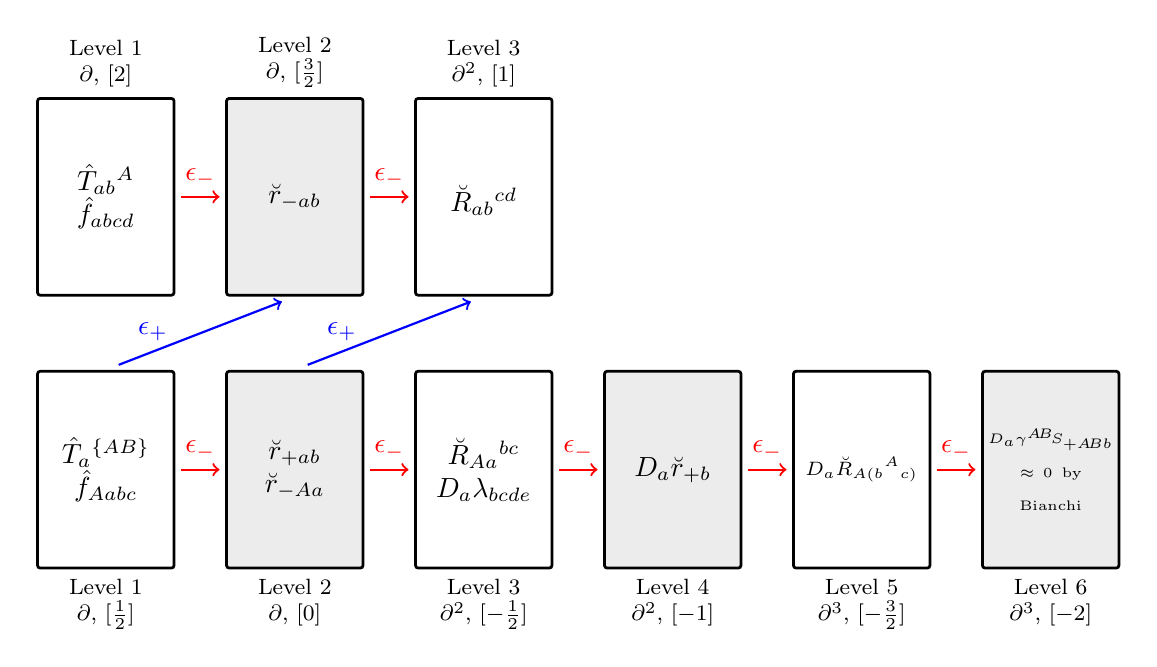
\begin{tikzpicture}
\draw (0,0) node [labels_up] {Level 1\\ $\partial$, [2] };
\draw (0,0) node (B1) [B,box_up] { $\hat T_{ab}{}^A$ \\ $\hat f_{abcd}$};

\def\x{2.4}
\draw (\x,0) node [labels_up] { Level 2\\ $\partial$, [$\tfrac32$]};
\draw (\x,0) node (F1) [F,box_up] {$\breve{r}_{-ab}$};

\draw (2*\x,0) node [labels_up] {Level 3 \\ $\partial^2$, [1] };
\draw (2*\x,0) node (B2) [B,box_up] {%
 \\ $\breve{R}_{ab}{}^{cd}$ \\ 
 };

% bottom row 
\begin{scope}[xshift =-2.4cm]
\draw (1*\x,-6) node [labels_down] { Level 1 \\ $\partial$, [$\tfrac12$]};
\draw (1*\x,-6) node (B1down) [B,box_down] {$\hat T_a{}^{\{AB\}}$\\$\hat f_{Aabc}$ };

\draw (2*\x,-6) node (F1labelsdown) [labels_down] {Level 2 \\ $\partial$, [0] };
\draw (2*\x,-6) node (F1down) [F,box_down] {$\breve{r}_{+ab}$ \\ $\breve{r}_{-Aa}$};

\draw (3*\x,-6) node [labels_down] { Level 3 \\ $\partial^2$, [$-\tfrac12$] };
\draw (3*\x,-6) node (B2down) [B,box_down] {%
$\breve{R}_{Aa}{}^{bc}$ \\
$D_a \lambda_{bcde}$};

\draw (4*\x,-6) node [labels_down] { Level 4 \\ $\partial^2$, [$-1$] };
\draw (4*\x,-6) node  (F2) [F,box_down] {$D_a \breve{r}_{+b}$};

\draw (5*\x,-6) node [labels_down] { Level 5 \\ $\partial^3$, [$-\tfrac32$]};
\draw (5*\x,-6) node (B3) [B,box_down] {\scriptsize $D_a\breve{R}_{A(b}{}^{A}{}_{c)}$	};

\draw (6*\x,-6) node [labels_down] { Level 6 \\ $\partial^3$, [$-2$]};
\draw (6*\x,-6) node (F3) [F,box_down] {\tiny $\! D_a\gamma^{A\!B}\!S_{+A\!B b}$ \\ $\approx 0$ by Bianchi};

\end{scope}

% putative bottomer row 
 \begin{comment}
\begin{scope}[xshift =-2.4cm]
\draw (1*\x,-10) node (llower) [labels_down] { $\partial$, [$-1$]};
\draw (1*\x,-10) node (Blambda1) [B,box_down] {$\lambda_{abcd}$ };

\draw (2*\x,-10) node [labels_down] {$\partial$, [$-\tfrac32$] };
\draw (2*\x,-10) node (Flambda1) [F,box_down] {$\breve{r}_{+a}$};

\draw (3*\x,-10) node [labels_down] { $\partial^2$, [$-2$] };
\draw (3*\x,-10) node (Blambda2) [B,box_down] {$\breve{R}_{A(b}{}^{A}{}_{c)}$ \\ $\breve{R}_{AB}{}^{bc}$};

\draw (4*\x,-10) node [labels_down] { $\partial^2$, [$-\tfrac52$] };
\draw (4*\x,-10) node  (Flambda2) [F,box_down] {\footnotesize
$S_{-AB}$};

\end{scope}
\end{comment}

%arrows
\draw[redarrows] (B1.east) -- (F1.west) node [midway,above] {$\epsilon_-$};
\draw[redarrows] (F1.east) -- (B2.west) node [midway,above] {$\epsilon_-$};
\draw[bluearrows] (B1down.north) -- (F1.south) node [pos=0.25,above] {$\epsilon_+$};
\draw[bluearrows] (F1down.north) -- (B2.south) node [pos=0.25,above] {$\epsilon_+$};
\draw[redarrows] (B1down.east) -- (F1down.west) node [midway,above] {$\epsilon_-$};
\draw[redarrows] (F1down.east) -- (B2down.west) node [midway,above] {$\epsilon_-$};
\draw[redarrows] (B2down.east) -- (F2.west) node [midway,above] {$\epsilon_-$};
\draw[redarrows](F2.east) -- (B3.west) node [midway,above] {$\epsilon_-$};
\draw[redarrows] (B3.east) -- (F3.west) node [midway,above] {$\epsilon_-$};
%


\end{tikzpicture}

\end{document}